\section{Examples of derivable functions}\label{sec:AppendixExamples}
To illustrate derivable functions, we present a series of examples, some of them will be useful later.

\noindent \begin{example}[Identity] For every type $\rSigma$, the identity function $x\in\rSigma\mapsto x\in\rSigma$ is derivable. This is achieved by induction on the types: the identity function over a finite set of elements is derivable since its domain is finite. %, and the identity function over $\llone$ is the first-order function $!$.
For every types $\rSigma$ and $\rGamma$, the identity
function over $\ranked{\rSigma+\rGamma}$ is the disjoint union of the co-projections $\ranked{\rSigma \to \rSigma + \rGamma}$ and $\ranked{\rGamma \to \rSigma + \rGamma}$. The
identity function over $\ranked{\rSigma \times \rGamma}$ is the pairing of the projections $\ranked{\rSigma \times \rGamma \to \rSigma}$ and $\ranked {\rSigma \times \rGamma \to \rGamma}$. The
identity function over $\ranked{\rSigma \otimes \rGamma}$ is the tensor product of the identity over $\rSigma$ and the identity over $\rGamma$. Finally,
the identity function over $\tmonad\rSigma$ and $\reduce k$ are constructed from the identity function over $\rSigma$ using the combinators $\tmonad$ and $\reduce k$ respectively.
\end{example}


\medskip
\noindent\begin{example}[Filter]\label{ex:filter} Consider the types $\rGamma, \rSigma$  where $\rGamma$ is a finite type of unary symbols. Consider the function:
$$ \ranked{f:\tmonad (\rSigma+\rGamma)\to\tmonad \rSigma}$$
which erases the elements of $\rGamma$ from the inupt tree. This function is well defined since erasing unary symbols does not break the tree structure of the input. 
Let us explain why this is a derivable function. 
Consider the basic functions $\ranked{\unit_\rSigma:\rSigma\to\tmonad\rSigma}$ and the constant function $\ranked{\mathsf{empty}:\rGamma\to\tmonad\rSigma}$ which associates to every element of $\rGamma$ the tree reduced to the variable $x_1$. Using the cases combinator, we get a tree in $\tmonad\tmonad\rSigma$, which we transform into a tree in $\tmonad \rSigma$ using the flattening function $\flatt_\rSigma$.
\end{example}


\medskip
\noindent \begin{example}[Pattern matching]\label{ex:patternMatching} 
\end{example}


\medskip
\noindent \begin{example}[Parent and sibling informations]  Let $\rGamma$ be a finite type. We define $\ranked{\rGamma_0}$  to be the ranked set obtained from $\rGamma$ by setting the arity of every element to $0$.  
\medskip
Consider the function:
$$\ranked{ \mathsf{Parent}: \tmonad \rGamma \to \tmonad (\rGamma\otimes (\rGamma+\bot)_0)}$$
which adds to every node of a term in $\tmonad \rSigma$ the label  of its parent if it has one and $\bot$ if it is the root.

% from  $(\rGamma\cup\bot)^{\leq n}$, whose lenght is the arity of the node, and such that the $i^{th}$ element of the  list is the symbol of its $i^{th}$ sibling if it has one, otherwise it is $\bot$.
Let us explain why $\ranked{\mathsf{Parent}}$ is derivable. 
\begin{enumerate}
\item For every symbol $a\in \rGamma$, consider the unary symbols $a_\#$ and $a_\$$.
We set $\ranked{\rGamma_\#}=\{a_\#\mid a\in\rGamma\}$ and $\ranked{\rGamma_\$}=\{a_\$\mid a\in\rGamma\}$.
Let $g$ be the following function:
 \begin{align*}
\ranked{  g: \rGamma} &\ranked{\to \tmonad(\rGamma+\rGamma_\#+\rGamma_\$)}\\
  a &\mapsto a_\#\tensorpair{a\tensorpair{a_\$\tensorpair{x_1},\dots,a_\$\tensorpair{x_{\mathsf{arity(a)}}}}}.
\end{align*}
The action of $\ranked{g}$ on a $\rGamma$ symbol looks like this:
\begin{center}
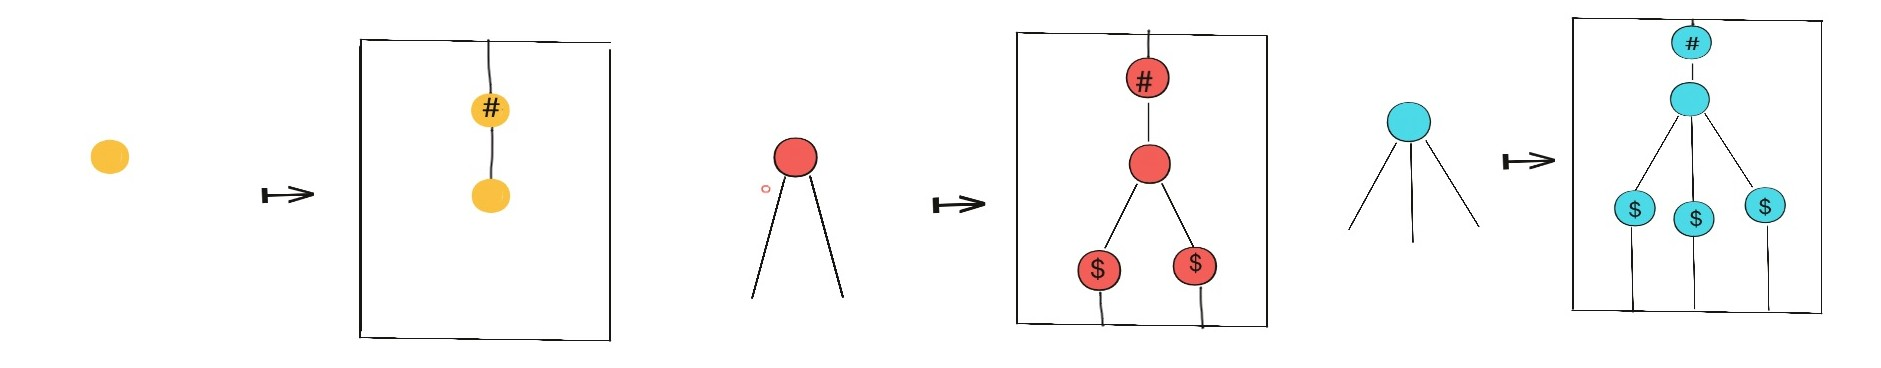
\includegraphics[scale=.15]{MyPic1.jpg}
\end{center}
\item We lift $\ranked{g}$ to the terms of $\tmonad \rGamma$ using the combinator $\tmonad$, then we apply a flattenig. After this operation, a term in $\tmonad\rGamma$ is transformed to a term in $\ranked{\tmonad(\rGamma+\rGamma_\#+\rGamma_\$)}$ this way:
\begin{center}
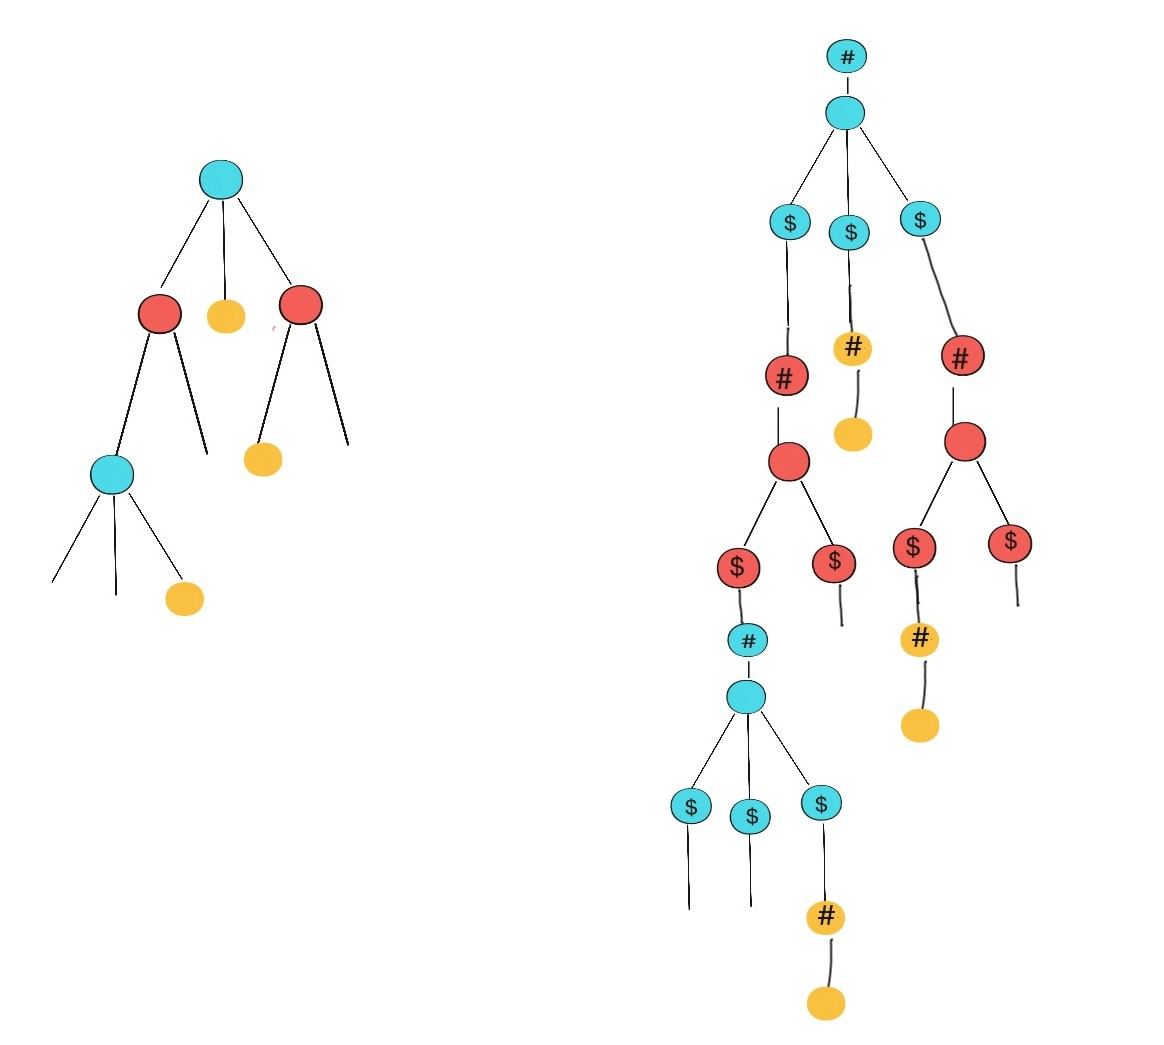
\includegraphics[scale=.15]{MyPic2.jpg}
\end{center}
\item We apply $\ancfact$, to separate the symbols of $\rGamma$ form the symbols of $\ranked{\rGamma_\#}$ and $\ranked{\rGamma_\$}$, we get then a term in $\ranked{\tmonad(\tmonad\rGamma+\tmonad(\rGamma_\#+\rGamma_\$))}$. Those terms look like this:
\begin{center}
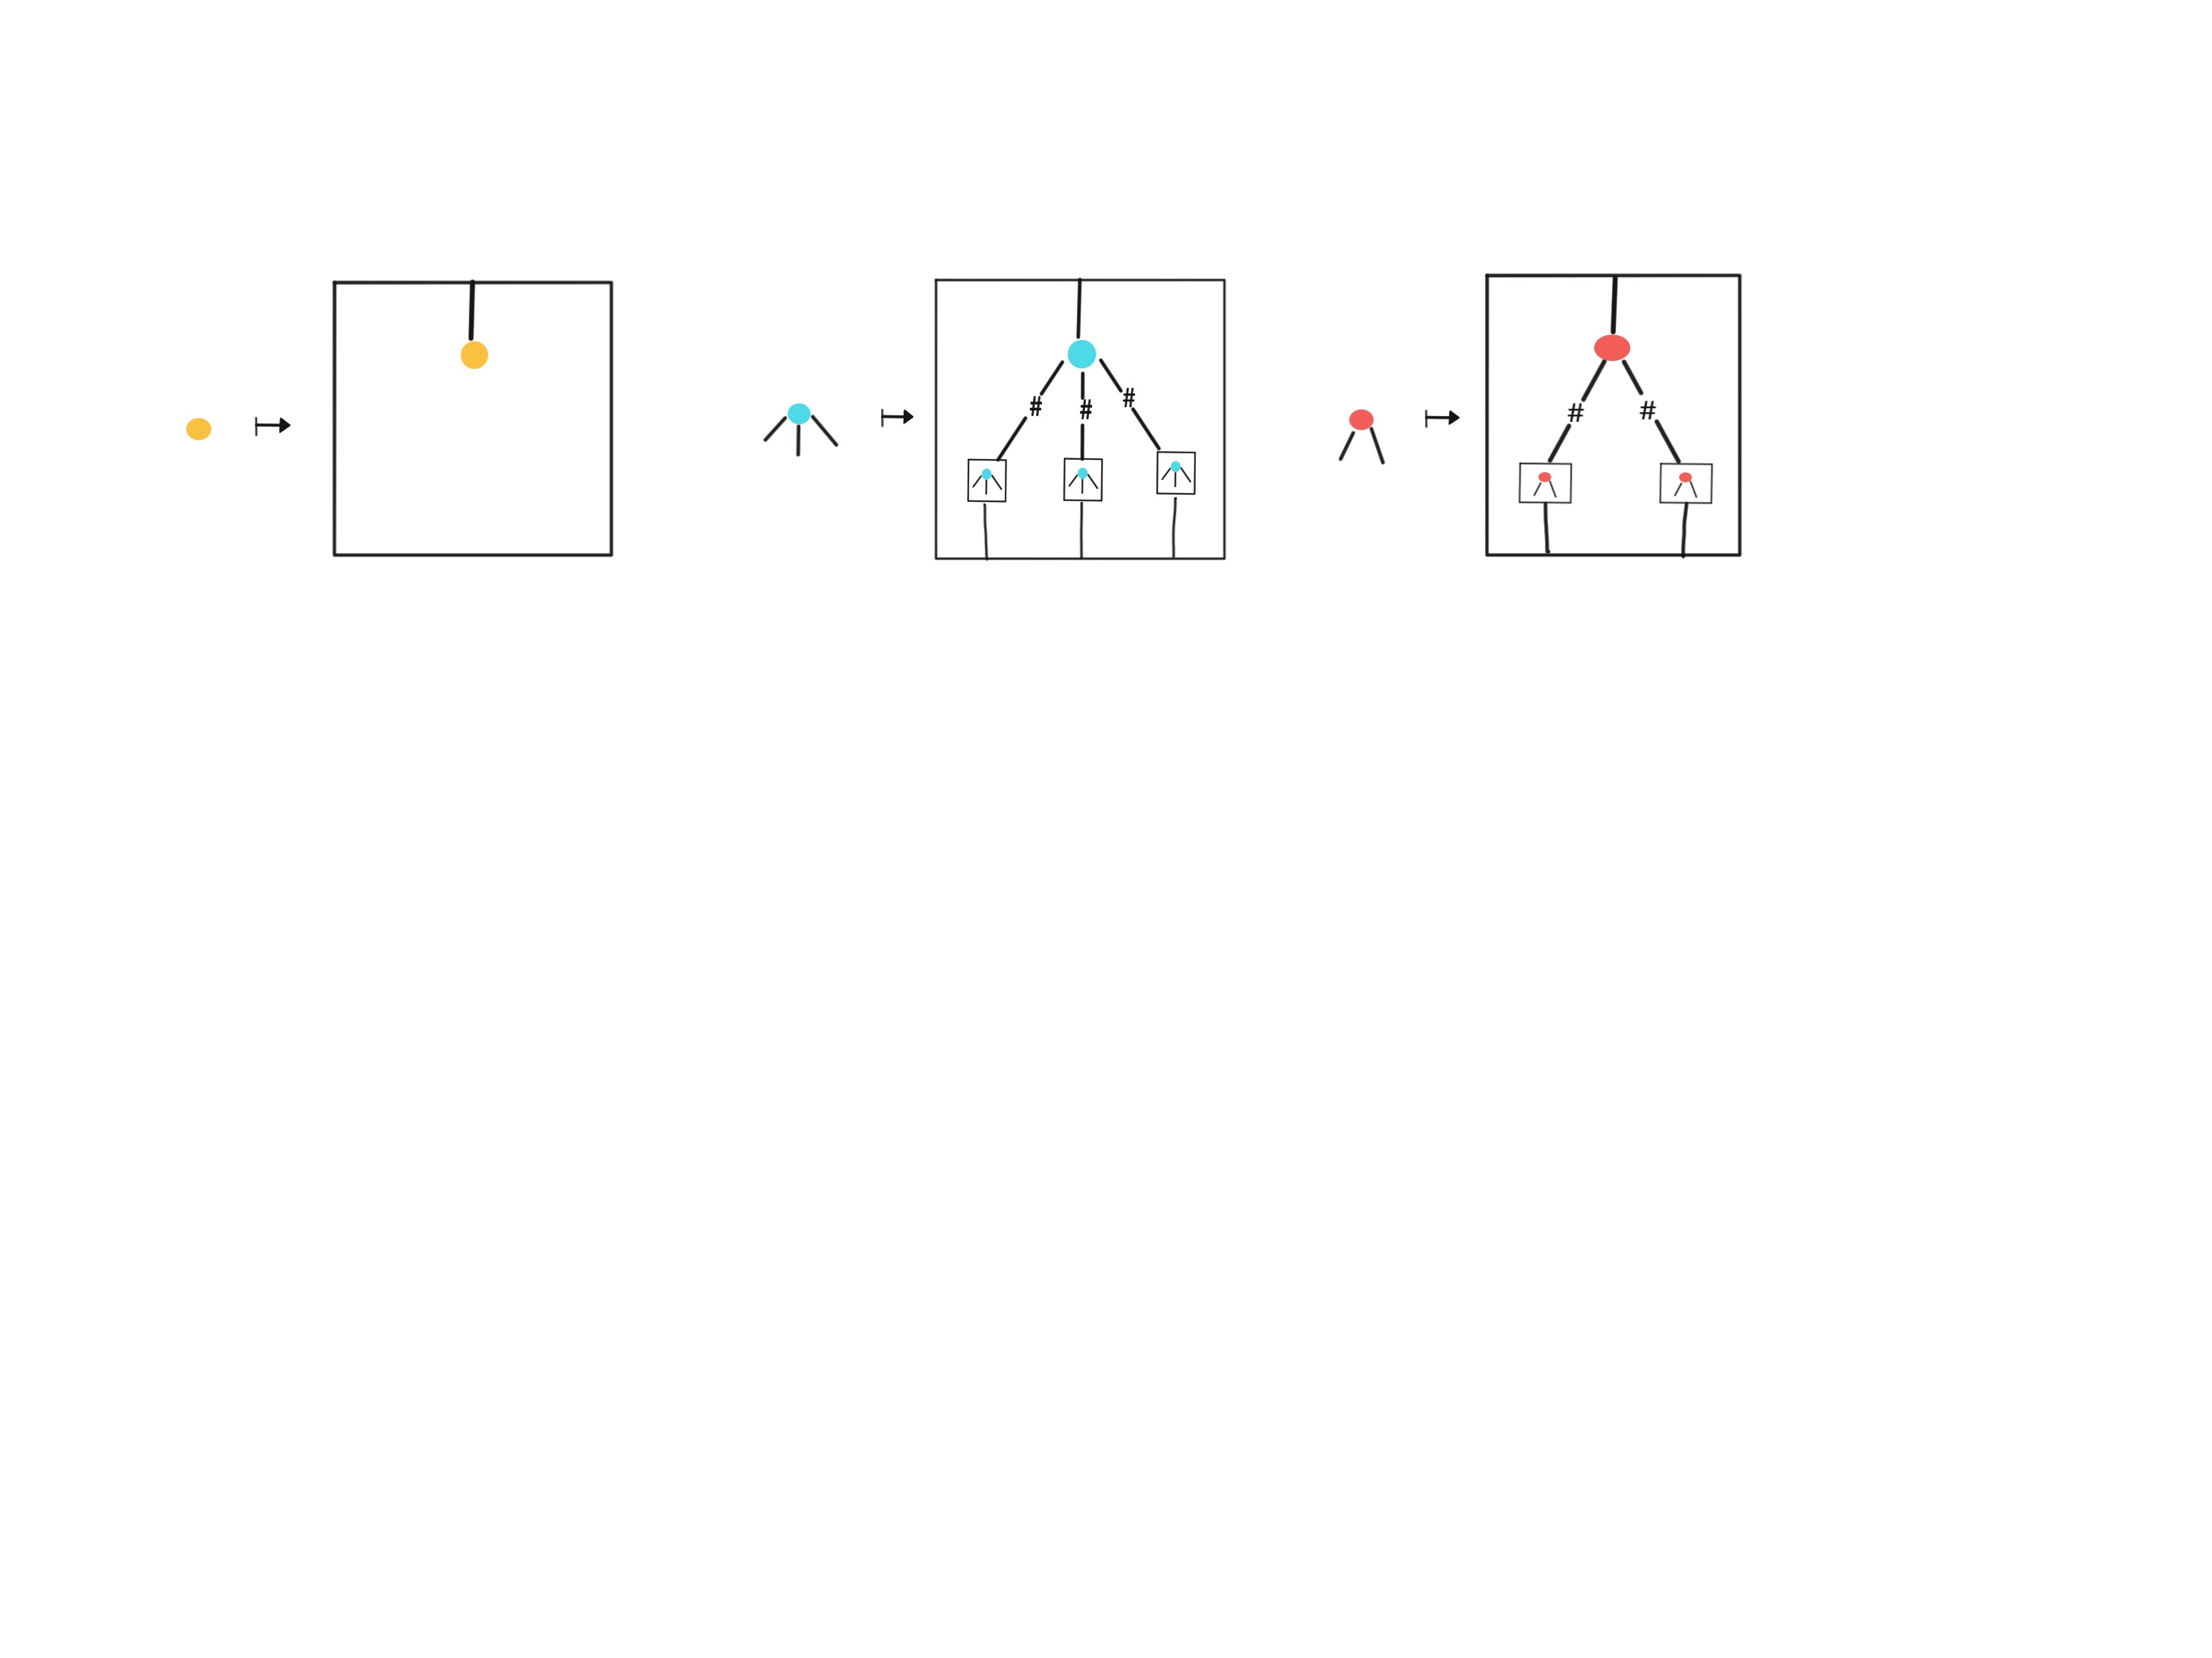
\includegraphics[scale=.15]{MyPic3.jpg}
\end{center}
\item Consider the function $\ranked{h:\tmonad(\rGamma_\#+\rGamma_\$)\to \tmonad(\rGamma_\#+\rGamma_\$)}$ which maps
\begin{align*}
a_\$\tensorpair{b_\#\tensorpair{x_1}} &\mapsto b_\$\tensorpair{a_\$\tensorpair{x_1}}&  a, b\in \rGamma\\
a_\$\tensorpair{x_1} & \mapsto  x_1&  a\in\rGamma
\end{align*}
and leaves the other terms unchanged. 
The function $\ranked{h}$ is derivable thanks to the pattern-matching construction of Example~\ref{ex:patternMatching}.

\item To the factors of type $\tmonad \rGamma$ we apply the identity function, and to the factors $\ranked{\tmonad(\rGamma_\#+\rGamma_\$)}$ we apply $\ranked{h}$. After that, we inject the factors into $\ranked{\tmonad(\rGamma+\rGamma_\#+\rGamma_\$)}$, then we apply a flattening to get terms in $\ranked{\tmonad(\rGamma+\rGamma_\#+\rGamma_\$)}$ having the form:
\begin{center}
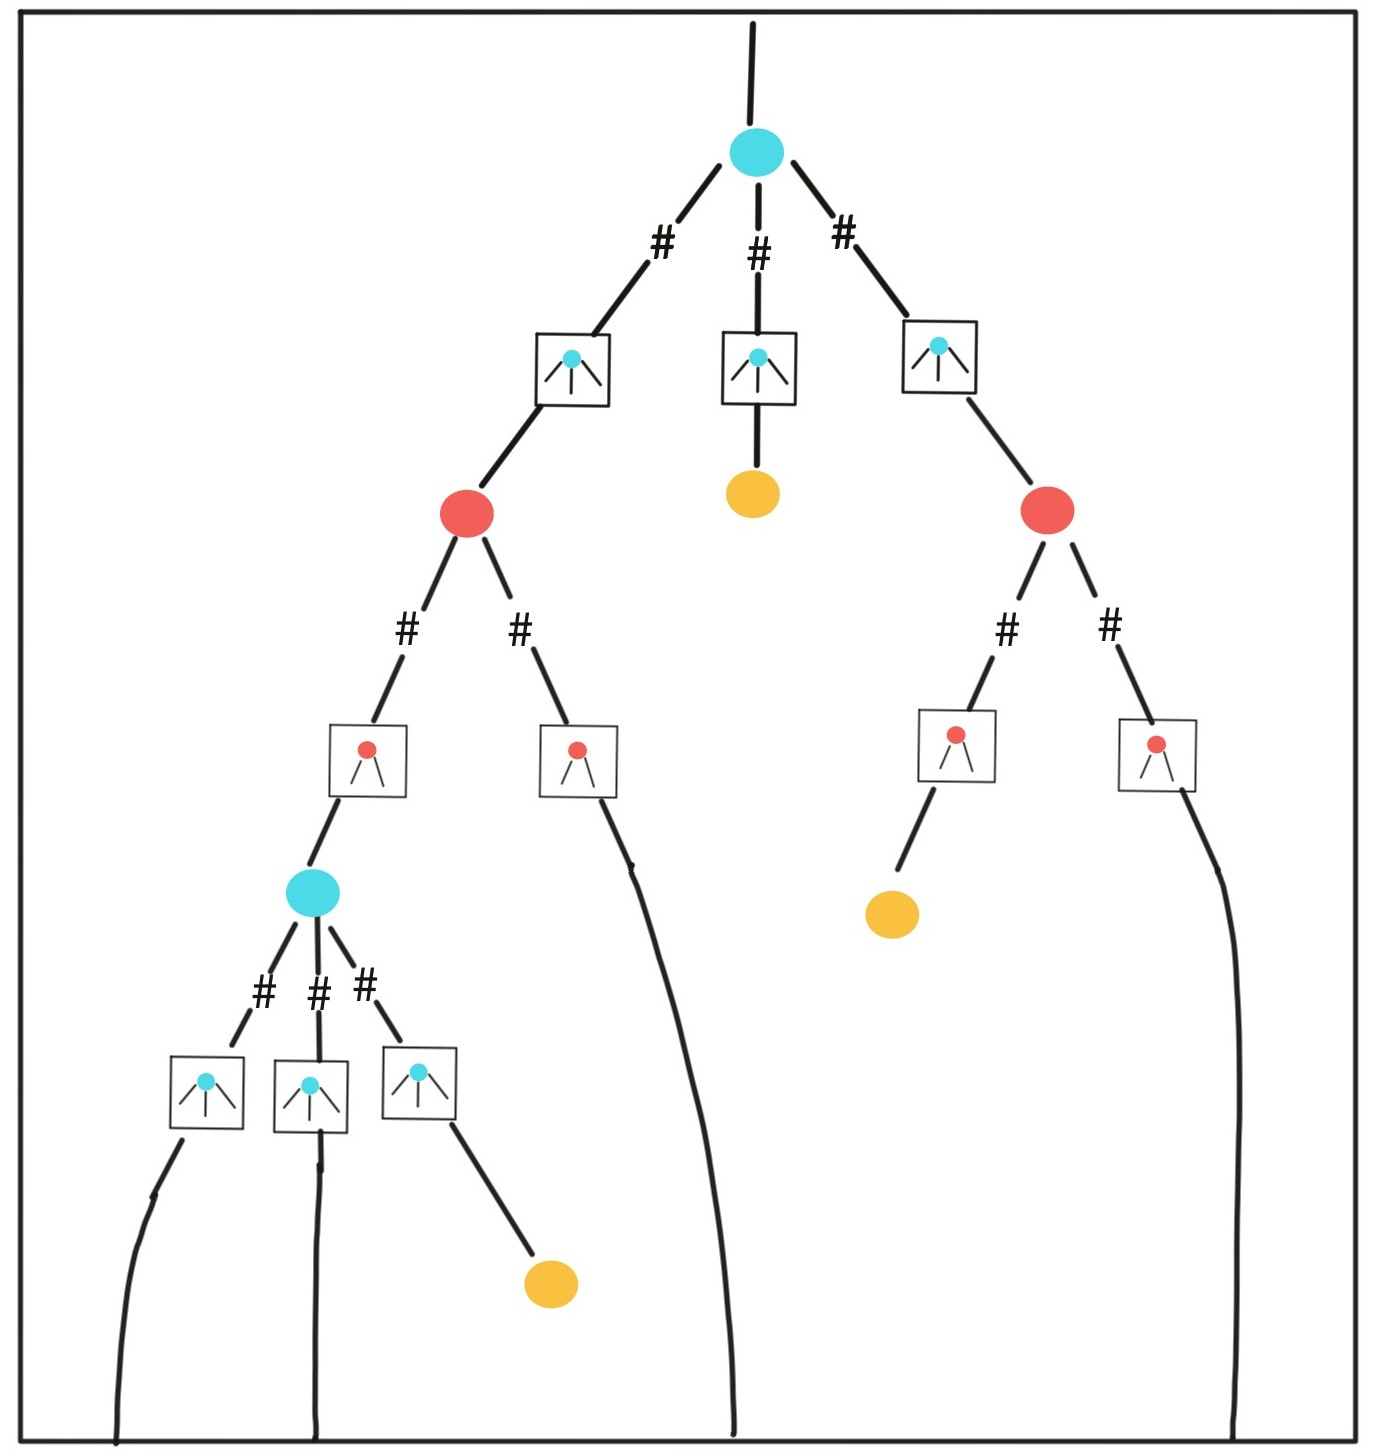
\includegraphics[scale=.15]{MyPic4.jpg}
\end{center} 
\item We apply $\ancfact$ to separate the symbols of $\ranked{\rGamma_\$}$ form the others. Doing so, every $\rGamma$ node ends up in the same factor as its parent (marked with $\$ $):
\begin{center}
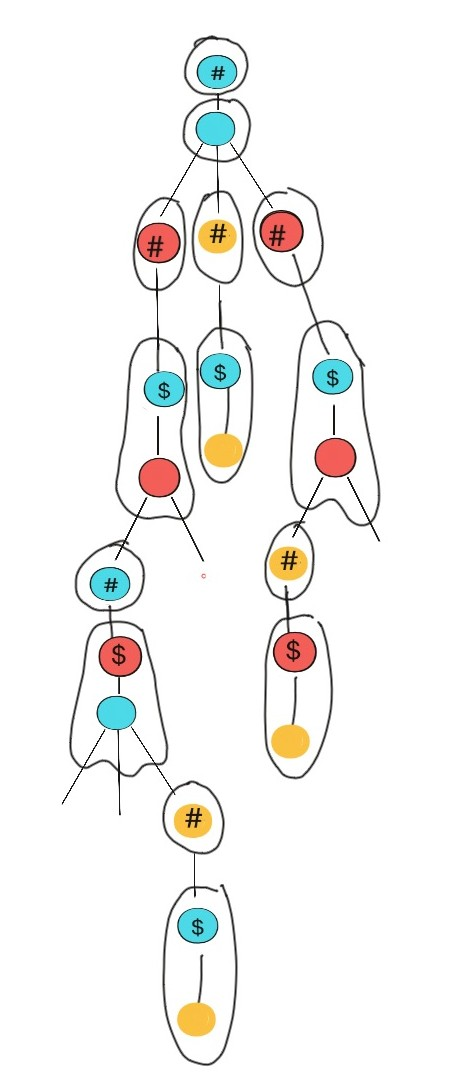
\includegraphics[scale=.15]{MyPic5.jpg}
\end{center}
\item Consider the function $\ranked{k:\tmonad(\rGamma+\rGamma_\#)\to \rGamma\otimes(\rGamma+\bot)_0+\tmonad(\rGamma+\rGamma_\#)}$ which maps
\begin{align*}
a\tensorpair{x_1,\dots,x_n} \mapsto \tensorpair{a,\bot} \\
b_\$\tensorpair{a\tensorpair{x_1,\dots,x_n}} \mapsto \tensorpair{a,b} 
\end{align*}
and leaves the terms other unchanged. We apply the function $\ranked{k}$ to the $\ranked{\tmonad(\rGamma+\rGamma_\#)}$
factors and the identity to the others. After several applications of injections and flattening, we get a term in $\ranked{\tmonad(\rGamma\otimes(\rGamma+\bot)_0+\rGamma_\#+\rGamma_\$+\rGamma)}$. We erase the symbols of $\ranked{\rGamma_\$}$ and $\ranked{\rGamma_\#}$  using the filter function from Example~\ref{ex:filter}, and obtain a term in $\ranked{\tmonad(\rGamma\otimes(\rGamma+\bot)_0+\rGamma)}$. 
We get rid of the symbols of $\rGamma$ in the output type, we apply any derivable function of type $\ranked{\rGamma\to \rGamma\otimes(\rGamma+\bot)_0}$, for example the one defined by:
\begin{align*}
a \mapsto \tensorpair{a,\bot}
\end{align*}
 Doing so we get the desired function.
\end{enumerate}
\medskip
If $\rGamma$ is a finite ranked set, we define $\ranked{\Gamma^*}$ as
$$\ranked{\coprod_{i \leq \text{ maximal arity in } \rGamma} \underbrace{\rGamma\otimes \cdots \otimes \rGamma}_{i\text{ times}}}$$
Now consider the function $$\ranked{\mathsf{Sibling}:\tmonad\rGamma\to \tmonad (\rGamma\otimes (\rGamma+\bot)^*_0)}$$ which taggs every node of a term in $\tmonad \rSigma$ by the list  of its children symbols. When a child is a port, it is marked by $\bot$ in the list.
The fuction $\ranked{\mathsf{Sibling}}$ is derivable. To see this, the same steps above can be followed, exept for steps 6 and 7 which should be adapted to this case. 
\end{example}



\medskip
\noindent  \begin{example}[Root and leaves] Let $\rSigma$ be a finite type and $f:\rSigma \to \rGamma$, $g: \rSigma \to \rGamma$ be derivable functions. The function $$\ranked{\mathsf{Root}_{f,g} : \tmonad\rSigma \to \tmonad\rGamma}$$
which applies $f$ to the root and $g$ to the rest of the tree is a derivable function.
 
To show this, we first start by applying the function $\ranked{\mathsf{Parent}:\tmonad\rSigma\to\tmonad(\rSigma\otimes(\rSigma+\bot)_0)}$. Doing so, the root can be distinghished from the other nodes since it will be tagged by $\bot$.  

The function $\ranked{h}$ defined by 
\begin{align*}
\ranked{h:\rSigma\otimes(\rSigma+\bot)_0}&\ranked{\to \rGamma}\\
  \tensorpair{a,\bot} &\mapsto f(a) \\
  \tensorpair{a,b} &\mapsto g(a) \text{ if } b\neq \bot.
\end{align*}
is derivable since its domain is finite. 
We lift $h$ to terms of $\tmonad\rGamma$ to conclude.


%We lift the function $ditribute_\otimes: \rSigma\otimes\rSigma^{\leq 1}\to  \rSigma\otimes\rSigma^{=0}+ \rSigma\otimes\rSigma^{= 1}$ to the trees of $\tmonad \rSigma\otimes\rSigma^{\leq 1}$ to get trees in $\tmonad (\)$.

\medskip
The function $$\ranked{\mathsf{Leaves}_{f,g} : \tmonad\rSigma \to \tmonad\rGamma}$$
 which applies $f$ to the leaves and $g$ to the rest of the tree is derivable. This is done using the same ideas as before, but invoquing the function $\ranked{\mathsf{Sibling}}$ instead of the function $\ranked{\mathsf{Parent}}$: leaves can be distingushed from the other nodes since they are tagged either by a list of $\bot$ or the empty list.
\end{example}

\medskip
\noindent\begin{example}[Descendent and ancestors] If $\rSigma$ is a finite type and $\rGamma\subseteq \rSigma$, then the functions 
\begin{itemize}
\item $\ranked{\mathsf{Descendant}_\rGamma: \tmonad \rSigma \to \tmonad (\rSigma+\rSigma)}$ which replaces the label of each node by its first or second copy, depending on whether it has a descendent in $\rGamma$,
\item $\ranked{\mathsf{Ancestor}_\rGamma: \tmonad \rSigma \to \tmonad (\rSigma+\rSigma)}$ which replaces the label of each node by its first or second copy, depending on whether it has a descendent in $\rGamma$,
\end{itemize}
are derivable.

To derive $\ranked{\mathsf{Descendant}_\rGamma}$, we start by applying the factorisation $$\ranked{\decfact: \tmonad\rSigma\to \tmonad(\tmonad\rGamma+\tmonad(\rSigma\setminus\rGamma))}$$ which regroups the elements of $\rSigma$ and the elements of $\ranked{\rSigma\setminus\rGamma}$ into factors, as in the following figure, where $\rGamma$ is represented by the blue nodes and $\ranked{\rSigma\setminus \rGamma}$ by the red ones:
\begin{center}
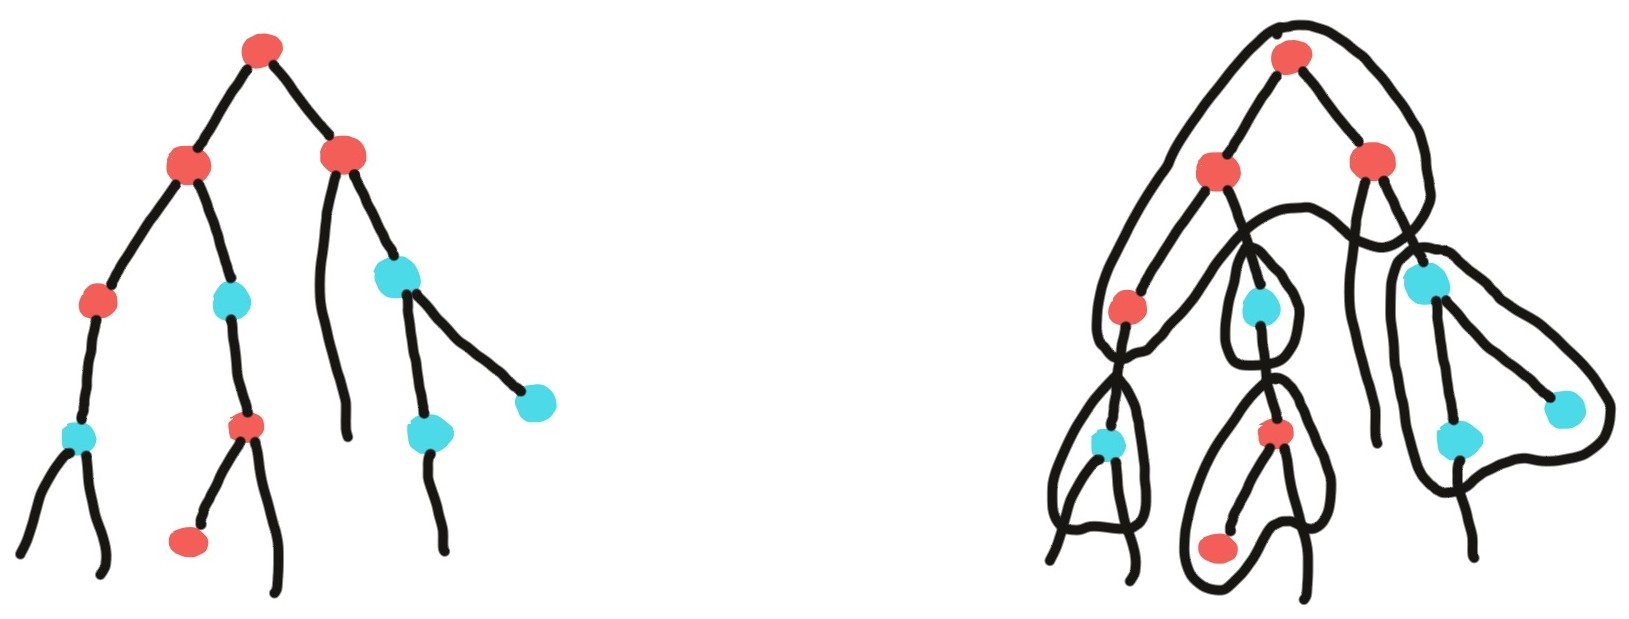
\includegraphics[scale=.15]{MyPic6.jpg}
\end{center}
Obviously, all the nodes of the $\Gamma$ factors have a descendant in $\rGamma$. 
In the $\ranked{\rSigma\setminus\rGamma}$ factors which are not leaves in the factorized term, all the nodes have a $\rGamma$ descendant in the original term. To show this, take $f$ to be one of these factors, and suppose by contradiction that one of its nodes does not have a descendant in $\rGamma$. By definition of $\ancfact$, all the elements of $f$ do not have a descendant in $\rGamma$ as well. Since $f$ is not a leaf, it has a child $g$. The factor $g$ cannot be a $\rGamma$
factor as the nodes of $f$ would have a descendant in $\rGamma$. The factor $g$ is then necessarily  a $\ranked{\rSigma\setminus \rGamma}$ factor. If a node of $g$ has a descendant in $\rGamma$, this would give a $\rGamma$ descendant to one of the node of $f$. Thus all the nodes of $g$ are in $\ranked{\rSigma\setminus \rGamma}$ and do not have a descendant in $\rGamma$, meaning that $f$ and $g$ are actually the same factor, which gives a contradiction. Finally, the $\ranked{\rSigma\setminus\rGamma}$ factors which are leaves do not have a descendant in $\rGamma$. With these observations, we can now implement $\mathsf{Descendant}_\rGamma$. 

Let us consider the functions 
$$\begin{array}{llll}
\ranked{\mathsf{Yes}_\rGamma :} & \rGamma &\ranked{\to} &\ranked{ \rSigma+\rSigma}\\
 \ranked{\mathsf{Yes}_{\ranked{\rSigma\setminus\rGamma}:}}& \ranked{\rSigma\setminus\rGamma}&\ranked{\to} &\ranked{ \rSigma+\rSigma}\\
\ranked{\mathsf{No}_{\ranked{\rSigma\setminus\rGamma}: }}&\ranked{\rSigma\setminus\rGamma} &\ranked{\to}& \ranked{ \rSigma+\rSigma}
\end{array}$$
which replaces the label of each node by its first copy for $\ranked{\mathsf{Yes}_\Gamma}$ and $\ranked{\mathsf{Yes}_{\rSigma\setminus\rGamma}}$, and by its second copy for $\ranked{\mathsf{No}_{\rSigma\setminus\rGamma}}$. The three functions are derivable as their domains are finite. 
Consider the functions 
\begin{align*}
\ranked{f} &\ranked{: \tmonad\rGamma+\tmonad(\rSigma\setminus\rGamma) \to \tmonad (\rSigma+\rSigma)}\\
&=\ranked{ \tmonad\mathsf{Yes}_\rGamma \text{ or } \tmonad\mathsf{No}_{\rSigma\setminus \rGamma}}\\
\ranked{g} &\ranked{: \tmonad\rGamma+\tmonad(\rSigma\setminus\rGamma) \to \tmonad (\rSigma+\rSigma)}\\
&=\ranked{ \tmonad\mathsf{Yes}_\rGamma \text{ or } \tmonad\mathsf{Yes}_{\rSigma\setminus \rGamma}} 
\end{align*}
The descendant function is obtained by applying $\ranked{\mathsf{leaves}_{f,g}}$ followed by a flattening.

To derive the function $\ranked{\mathsf{Ancestor}_\Gamma}$, we apply first a the factorisation
$$\ranked{\ancfact: \tmonad\rSigma\to \tmonad(\tmonad\rGamma+\tmonad(\rSigma\setminus\rGamma))}$$ which regroups the elements of $\rSigma$ and the elements of $\ranked{\rSigma\setminus\rGamma}$ into factors depending on whether they have the same descendant of the same type. Here is an example,  where $\rGamma$ is represented by the blue nodes and $\ranked{\rSigma\setminus \rGamma}$ by the red ones:
\begin{center}
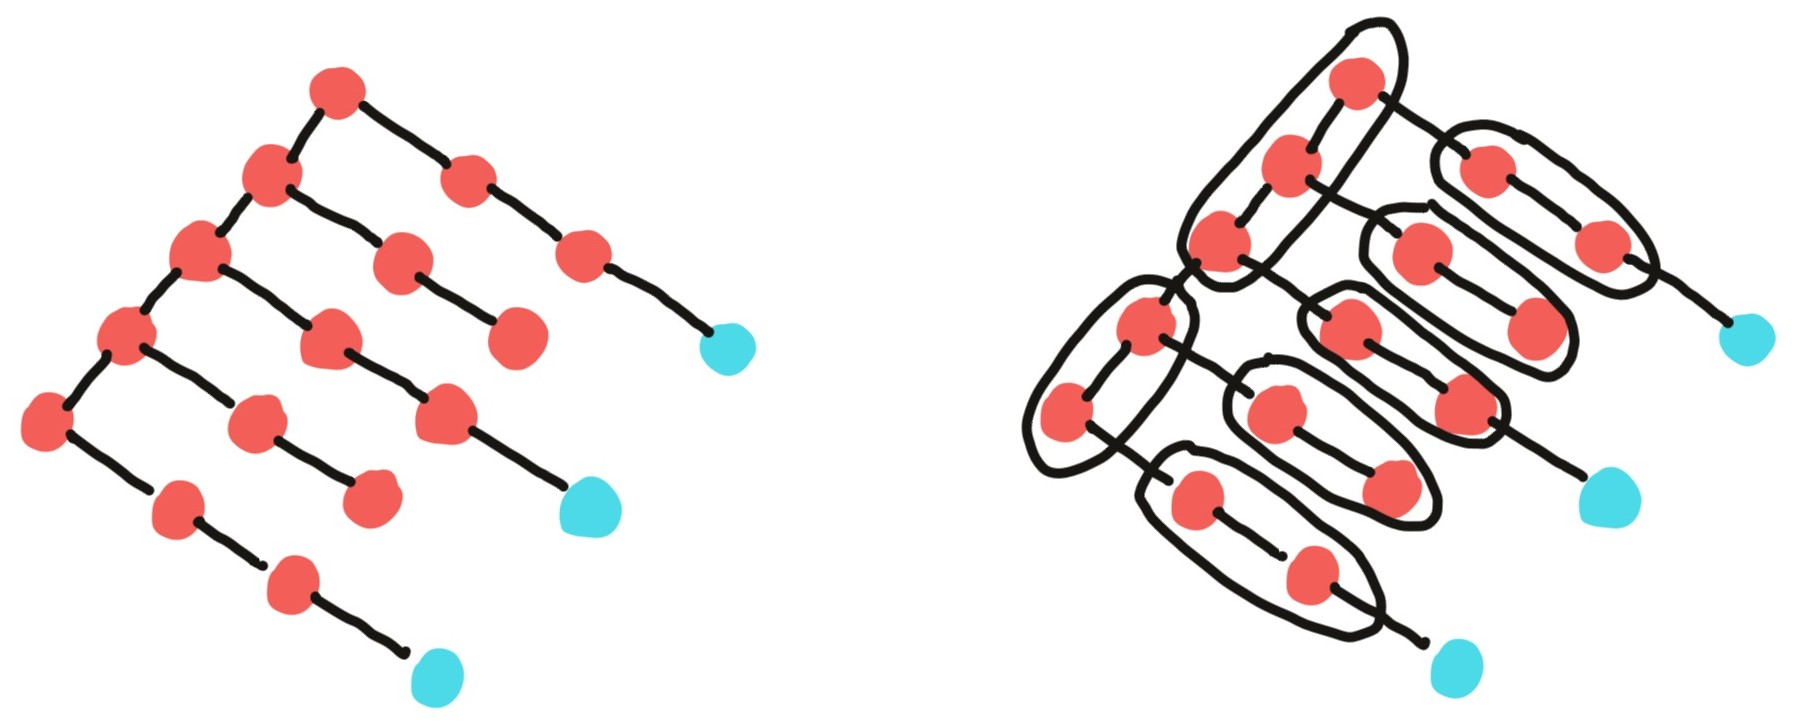
\includegraphics[scale=.15]{MyPic7.jpg}
\end{center}
Using similar arguments as befor, we can conclude that:
\begin{itemize}
\item The nodes inside $\rGamma$ factors have $\rGamma$ ancestors.  
\item If a $\ranked{\rSigma\setminus\rGamma}$ factor is the root of the factorized term, then its nodes do not have a $\rGamma$ ancestor.
\item   If a $\ranked{\rSigma\setminus\rGamma}$ factor is not the root of the factorized term, then its nodes do have a $\rGamma$ ancestor.
\end{itemize}
The ancestor function is obtained by applying $\ranked{\mathsf{root}_{f,g}}$ followed by a flattening.

Note here the importance of the basic function $\decfact$. If we had only the factorisation $\ancfact$, we would not be able to separate (at least easily) the red blocks having a blue descendent from the others in the figure above.  
\end{example}
%\medskip
%\noindent \begin{example}[Characteristic function of a finite type]
%Let $\rSigma, \Delta\in \Tt$ and suppose that $\rSigma$ is finite. 
%The order-preserving function $\chi_\rSigma:\Delta\to \llzero+\llone$ which satisfies $\chi_\rSigma(s)\in \llone$ if and only if $s\in \rSigma$ is a first-order tree function. 
%\end{example}
%\medskip
%\noindent \begin{example}[If then else] Suppose that $f : \rSigma \to \llzero+\llone$ and $g_0, g_1 : \rSigma \to\rGamma$ are first-order tree functions. Then the function:
% \begin{align*}
%  g\colon \rSigma &\to \rGamma \\
%  x &\mapsto g_0(x)  \text{ if } f(x)\in\llzero\\
%  x &\mapsto g_1(x)  \text{ if } f(x)\in\llone.
%\end{align*}
% is also a first-order tree function. This is done as follows. On input!!
%$x\in\rSigma$, we first apply the pairing of f and the identity function, yielding a result:
%$$ (f(x),x)\in(\llzero+\llone)\times\rSigma$$
%Next we apply the function distribute, transforming the type into:
%$$ \llzero\times\rSigma+\llone\times\rSigma$$
%To this result we apply the disjoint union $h_0 + h_1$ where $h_0:\llzero\times\rSigma\to \rGamma$ and
%$h_01:\llone\times\rSigma\to \rGamma$ are defined by $h_i=\pi_2(id_i,g_i)$, where $id_0$ and $id_1$ are the identity function on $\llzero$ and $\llone$ respectively, yielding the desired result.
%\end{example}

